%% LaTeX-Beamer template for KIT design
%% by Erik Burger, Christian Hammer
%% title picture by Klaus Krogmann
%%
%% version 2.1
%%
%% mostly compatible to KIT corporate design v2.0
%% http://intranet.kit.edu/gestaltungsrichtlinien.php
%%
%% Problems, bugs and comments to
%% burger@kit.edu

\documentclass[18pt]{beamer}

%% SLIDE FORMAT

% use 'beamerthemekit' for standard 4:3 ratio
% for widescreen slides (16:9), use 'beamerthemekitwide'
% for widescreen slide without sidebar use 'beamerthemekitwidenosidebar'

\usepackage{xkeyval}
\usepackage{todonotes}
\presetkeys{todonotes}{inline}{}
\usepackage{templates/beamerthemekit}
\usepackage{tabularx}
%\usepackage{templates/beamerthemekitwide}
%\usepackage{templates/beamerthemekitwidenosidebar}

% use this to disable the latex beamer navigation symbols
%\beamertemplatenavigationsymbolsempty


%% TITLE PICTURE

% if a custom picture is to be used on the title page, copy it into the 'logos'
% directory, in the line below, replace 'mypicture' with the 
% filename (without extension) and uncomment the following line
% (picture proportions: 63 : 20 for standard, 169 : 40 for wide
% *.eps format if you use latex+dvips+ps2pdf, 
% *.jpg/*.png/*.pdf if you use pdflatex)

%\titleimage{images/}

%% TITLE LOGO

% for a custom logo on the front page, copy your file into the 'logos'
% directory, insert the filename in the line below and uncomment it

\titlelogo{2_TecO_Logo_m}

% (*.eps format if you use latex+dvips+ps2pdf,
% *.jpg/*.png/*.pdf if you use pdflatex)

%% TikZ INTEGRATION

% use these packages for PCM symbols and UML classes
% \usepackage{templates/tikzkit}
% \usepackage{templates/tikzuml}

% the presentation starts here

\title[]{Klassifikation von respiratorischen Ereignissen mit \\ Earables und maschinellem Lernen}
\subtitle{}
\author{David Laubenstein}

\institute{Institut für Telematik: Pervasive Computing Systems / TECO}

% Bibliography

\usepackage[citestyle=authoryear,bibstyle=numeric,hyperref,backend=biber]{biblatex}
\addbibresource{templates/example.bib}
\bibhang1em

\begin{document}

% change the following line to "ngerman" for German style date and logos
\selectlanguage{english}

%title page
\begin{frame}
\titlepage
\end{frame}

%table of contents
\begin{frame}{Outline/Gliederung}
\tableofcontents
\end{frame}

\section{Grundlagen}
\subsection{Problem}
\begin{frame}{Problem}
    \includegraphics[scale=0.4]{../Proposal/logos/was-passiert-bei-schlafapnoe}
    %\textit{\cite{becker2008a}}
\end{frame}

\begin{frame}{Problem}
    \begin{center}
        \includegraphics[scale=0.12]{../Proposal/logos/sleepLabor}
    \end{center}
\end{frame}

\subsection{Idee}
\begin{frame}{Idee}
%insert picture from Earbuds for solution to diagnose this 
    \begin{columns}[T] % align columns
	\begin{column}{.48\textwidth}
	    \includegraphics[scale=0.15]{../Proposal/logos/esense}
	\end{column}%
	\hfill%
	\begin{column}{.48\textwidth}
	    \includegraphics[scale=0.25]{../Proposal/logos/esense2}
	\end{column}%
	\end{columns}
	Vorteil:
	\begin{itemize}
		\item Test kann unkompliziert zuhause durchgeführt werden
		\item Sensoren bereits heute in Kopfhörern vorhanden (Apple AirPods)
	\end{itemize}
\end{frame}

\subsection{Idee}
\begin{frame}{Idee}
Erstellung eines Datensatzes zur Klassifikation
\begin{itemize}
    \item eSense-Earpods mit IMU
    \item Ground-Truth: Polysomnographie-Gerät
\end{itemize}

\begin{center}
    \begin{columns}
        \begin{column}{.6\textwidth}
           \includegraphics[scale=0.25]{images/study/psg_system_flow}
        \end{column}
        \begin{column}{.39\textwidth}
           \includegraphics[scale=0.16]{images/study/psg_system_picture} 
        \end{column}
    \end{columns}
\end{center}
\end{frame}

\section{Nutzerstudie}
\begin{frame}{Nutzerstudie$/$ Datensatz}
\begin{itemize}
    \item Nutzerstudie
    \begin{itemize}
        \item 7 Personen 
        \item 3 Positionen (Bauch, Seite, Rücken)
    \end{itemize}
    \item Was wird aufgezeichnet?
    \begin{itemize}
        \item eSense-Earpods (\textbf{IMU, Mikrofon})
        \item PSG-System
        \begin{itemize}
            \item Pulssensor am Finger
            \item Bauch- und Brustkorbsignal
            \item Drucksignal (Nase)
            \item Bewegungssignal
            \item Sauerstoffsättigung \& Sauerstoffgehalt
            \item Schnarchmikrofon
            \item Bewegungssignal
            \item Lichtsignal
            \item EDF Informationen
        \end{itemize}
    \end{itemize}
\end{itemize}
\end{frame}

\begin{frame}{Ablauf der Nutzerstudie}
    \includegraphics[scale=0.45]{images/study/study_flow2.pdf}
\end{frame}

\begin{frame}{Ablauf der Nutzerstudie}
    %\includegraphics[0.25]{images/study/study_flow2.pdf}
    \begin{center}
        \begin{columns}[T] % align columns
            \begin{column}{.33\textwidth}
                \centering
                \includegraphics[scale=0.1]{images/app/connect_success.PNG}
            \end{column}%
            \hfill%
            \begin{column}{.33\textwidth}
                \centering
                \includegraphics[scale=0.1]{images/app/measurement_details.PNG}
            \end{column}%
            \hfill%
            \begin{column}{.33\textwidth}
                \centering
                \includegraphics[scale=0.1]{images/app/measurement_timer_02.png}
            \end{column}%
        \end{columns} 
    \end{center}
\end{frame}

\begin{frame}{Beispielbilder der Nutzerstudie}
    \begin{center}
        \begin{columns}[T]
            \begin{column}{.49\textwidth}
                \centering
                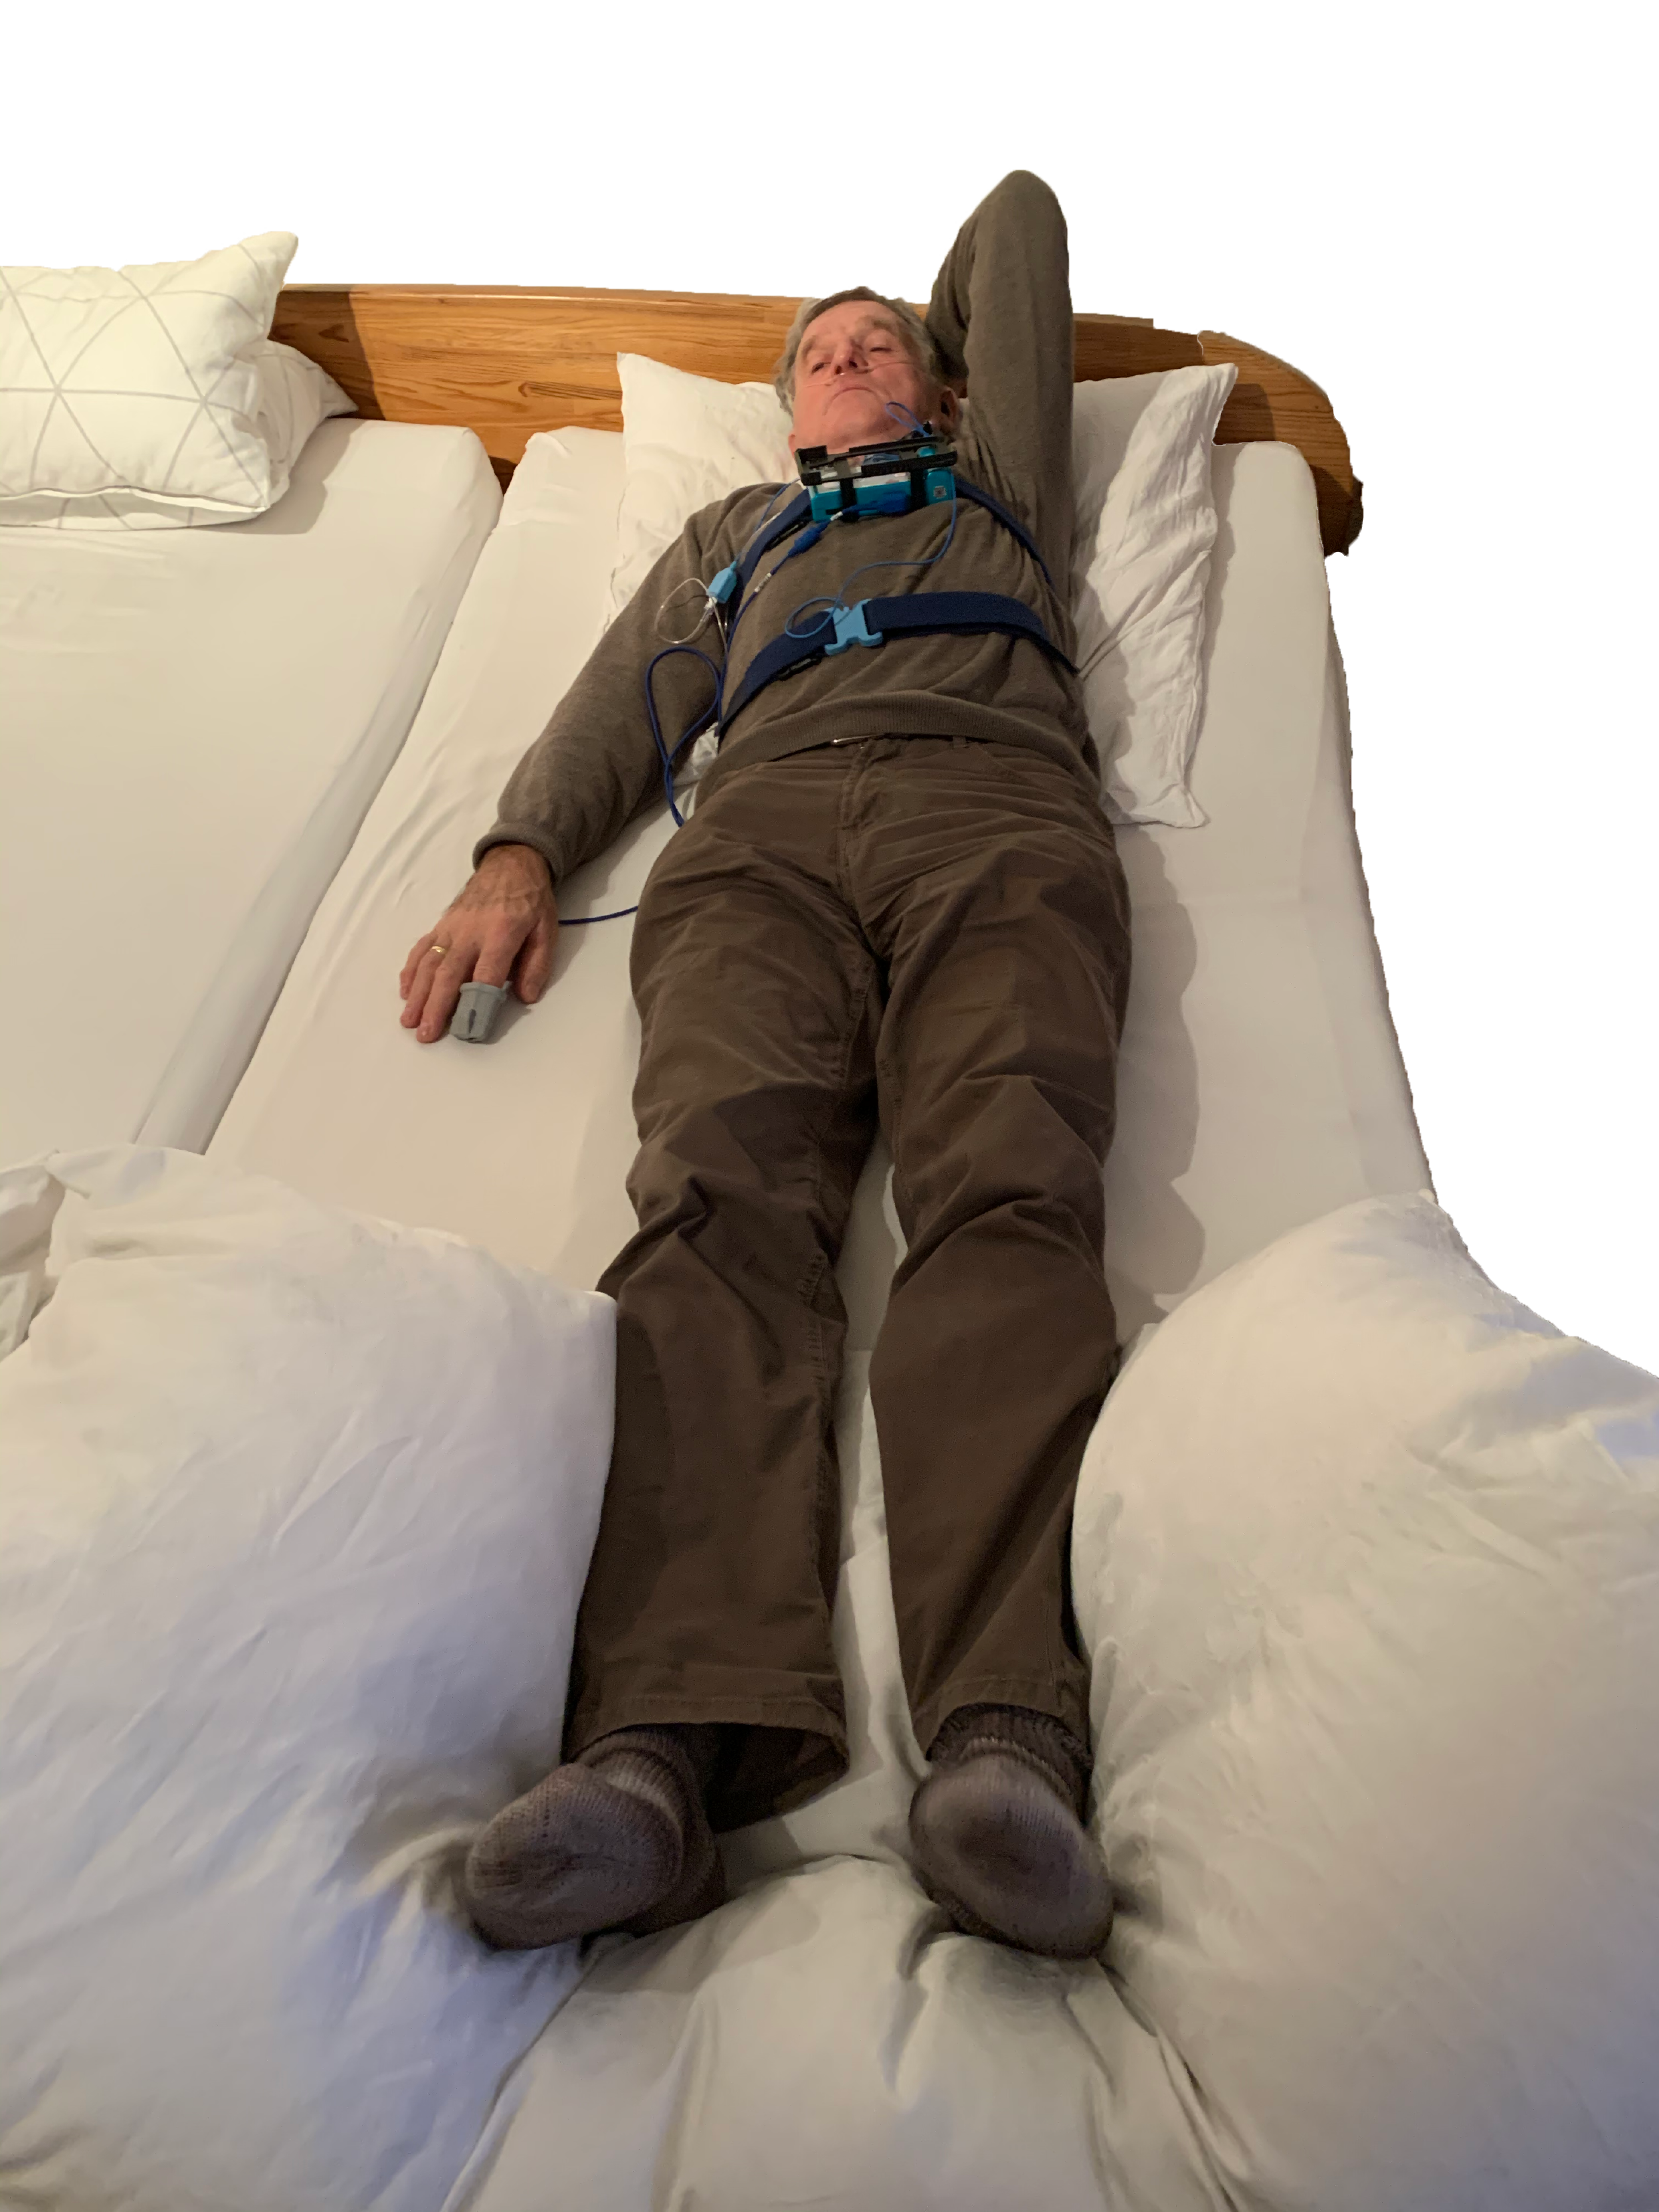
\includegraphics[scale=0.23]{images/study/study_proband_2_clean.png}
            \end{column}
            \hfill%
            \begin{column}{.49\textwidth}
                \centering
                \includegraphics[scale=0.12]{images/study/study_proband_clean2.png}
            \end{column}
        \end{columns}
    \end{center}
\end{frame}

\begin{frame}{Erste Resultate}
    \begin{center}
        \includegraphics[scale=0.16]{images/data_analyzation/compare_raw_signal_with_flowDr_2.png}
    \end{center}
\end{frame}

\section{Klassifikation}
\begin{frame}{Klassifikation / Idee}
\begin{itemize}
    \item Teile Messung in \textit{Fenster} auf.
    \begin{itemize}
        \item Länge: 5 bzw. 10 Sekunden
        \item Verschiebung: 1 Sekunde bzw 5, 10 Sekunde bei keiner Überlappung
    \end{itemize}
    \item Pro \textit{Fenster} werden Features berechnet.
    \begin{itemize}
        \item Mittels \texttt{tsfresh} werden ca. 6000 Features berechnet.
    \end{itemize}
    \item Klassifikation anhand der Features
    \begin{itemize}
        \item Evaluation mit dem Kreuzvalidierungsverfahren
        \begin{itemize}
            \item Within Subject
            \item Leave One Subject Out (LOSO)
        \end{itemize}
    \end{itemize}
\end{itemize}
\end{frame}

\begin{frame}{Within Subject}
    \begin{tabular}{|c|c|c|c|c|c|}
        \hline
        \textbf{Verfahren} & \textbf{Positionen} & \textbf{Score} & \textbf{Score} & \textbf{Score} & \textbf{Score} \\ 
        & & $w=5s$ & $w=5s$ & $w=10s$ & $w=10s$ \\
        & & $d=1s$ & $d=5s$ & $d=1s$ & $d=10s$ \\
        \hline
        Random Forest & Alle &  0.87 & 0.74 & 0.89 & 0.71 \\ 
        & Rücken & 0.85 & 0.67 & 0.93 & 0.57 \\
        & Seite  & 0.86 & 0.72 & 0.89 & 0.75 \\
        & Bauch  & 0.90 & 0.85 & 0.92 & 0.66 \\ \hline
        XG Boost  & Alle & 0.88 & 0.70 & 0.92 & 0.76 \\ 
        & Rücken & 0.89 & 0.67 & 0.95 & 0.62 \\
        & Seite  & 0.90 & 0.78 & 0.92 & 0.48 \\
        & Bauch  & 0.90 & 0.75 & 0.95 & 0.63 \\ \hline
        SVM & Alle& 0.54 & 0.48 & 0.65 & 0.42 \\ 
        & Rücken & 0.60 & 0.67 & 0.72 & 0.46 \\
        & Seite  & 0.57 & 0.38 & 0.63 & 0.5 \\
        & Bauch  & 0.61 & 0.41 & 0.67 & 0.4 \\
        \hline
    \end{tabular}
\end{frame}

\begin{frame} {Leave One Subject Out}
    Person 6: XGBoost mit einer Fenstergröße von 10\textit{s} und einer Verschiebung von 1\textit{s}.
    \begin{center}
        \includegraphics[scale=0.29]{images/evaluation/loso_10sec/xg_boost_loso/XGBoost(LeaveOneSubjectOutPerson6Back).png}
    \end{center}
    \begin{center}
        \includegraphics[scale=0.29]{images/evaluation/loso_10sec/xg_boost_loso/XGBoost(LeaveOneSubjectOutPerson6Side).png}
    \end{center}
    \begin{center}
        \includegraphics[scale=0.29]{images/evaluation/loso_10sec/xg_boost_loso/XGBoost(LeaveOneSubjectOutPerson6Stomach).png}
    \end{center}
\end{frame}

\begin{frame} {Leave One Subject Out}
    Person 8: XGBoost mit einer Fenstergröße von 10\textit{s} und einer Verschiebung von 1\textit{s}.
    \begin{center}
        \includegraphics[scale=0.29]{images/evaluation/loso_10sec/xg_boost_loso/XGBoost(LeaveOneSubjectOutPerson8Back).png}
    \end{center}
    \begin{center}
        \includegraphics[scale=0.29]{images/evaluation/loso_10sec/xg_boost_loso/XGBoost(LeaveOneSubjectOutPerson8Side).png}
    \end{center}
    \begin{center}
        \includegraphics[scale=0.29]{images/evaluation/loso_10sec/xg_boost_loso/XGBoost(LeaveOneSubjectOutPerson8Stomach).png}
    \end{center}
\end{frame}

\section{Aussicht}
\begin{frame}{Potenzial / Aussicht}
    \begin{center}
        \includegraphics[scale=0.25]{images/futureWork/pulseSpo2_edited.png}
    \end{center}
    \begin{itemize}
        \item Betrachtung von Puls- und $SpO_2$-Signalen.
        \item Kann mittels des \textit{Cosinuss One}-Earpods ermittelt werden.
    \end{itemize}
\end{frame}

\begin{frame} {Potenzial / Aussicht}
    \begin{itemize}
        \item Klassifikation mittels der Betrachtung vorangehender und nachfolgender \textit{Fenster}.
        \begin{itemize}
            \item z.B LSTM
        \end{itemize}
        \item Einbeziehung der Nutzerinformationen (Gewicht, Geschlecht)
    \end{itemize}
\end{frame}

\begin{frame} {Zusammenfassung}    
    \tableofcontents
\end{frame}

\appendix
%\begin{frame}{test}
%    \todo{Add test asdf}
%\end{frame}
%\beginbackup

\begin{frame}[allowframebreaks]{References}
\printbibliography
\end{frame}

%\backupend

\end{document}
